%archivo_indice.tex
\chapter{Anexos}
	\section{Sistemas operativos}
	El desarrollo del proyecto de memoria tuvo como fin un aplicación para el sistema operativo iOS. Para esto fue necesario utilizar las herramientas dispuestas por Apple Inc.
		\subsection{OSX}
La décima versión del sistema operativo para computadores Macintosh, la X se refiere al numero romano 10. Esta versión posee un micronúcleo Mach, junto a servicios de sistema operativo de tipo UNIX basados en FreeBSD.
Las aplicaciones para OSX se desarrollan utilizando \textbf{Cocoa} API, la interfaz de programación de aplicaciones orientada a objetos.
\subsubsection{Xcode}
Para este proyecto se utilizó el entorno de desarrollo \textbf{Xcode}, el cual está solamente disponible para OSX.\\

Xcode se puede obtener desde la tienda de aplicaciones de OSX, el repositorio que integra el mismo sistema de pago utilizado en la tienda de música digital iTunes Store (fig. \ref{fig:xcode-appstore}).
\begin{figure}[H]
	\centering
	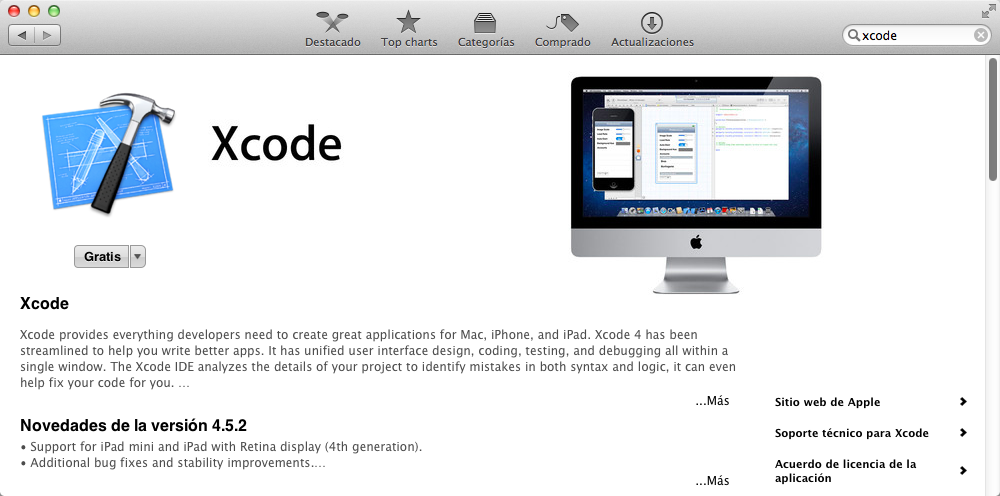
\includegraphics[scale=0.41]{imgs/xcode-appstore.png} 
	\caption{Xcode disponible gratis en la \textbf{App Store}, la tienda de aplicaciones para OSX}
	\label{fig:xcode-appstore}
\end{figure}  
%		os x, se empezó el desarrollo en lion, migración de xcode 3 a 4, inestabilidad
%		explicar como se usa  itunes con ios
		\subsection{iOS}
Sistema operativo para dispositivos móviles, originalmente fue desarrollado para iPhone, sin embargo se ha utilizado en nuevos productos de Apple como iPod Touch, iPad, y el Apple TV. Su caracteristica principal es la interfaz de usuario basada en manipulación de gestos táctiles por parte del usuario, es decir pellizcos, deslizamientos o toques con los dedos.\\

iOS deriva de Mac OSX en su arquitectura de diseño, utilizando también el mismo micronucleo Mach basado en FreeBSD: Darwin.\\

El desarrollo de sus aplicaciones se realiza con \textbf{Cocoa Touch} API (fig. \ref{fig:ios-cocoatouch}).
\begin{figure}[H]
	\centering
	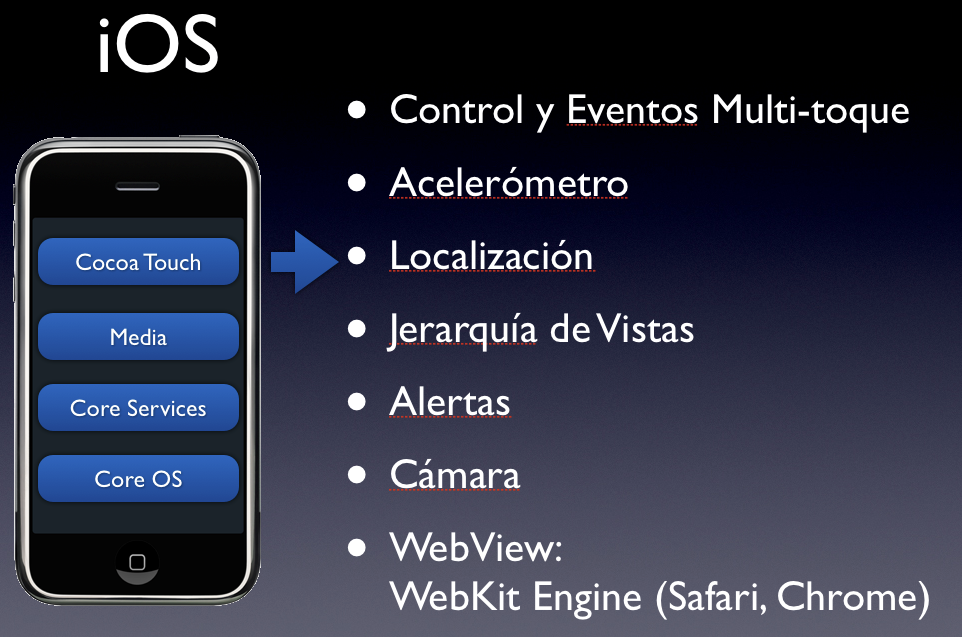
\includegraphics[scale=0.35]{imgs/ios-cocoatouch.png} 
	\caption{Caracteristicas de la API Cocoa Touch.}
	\label{fig:ios-cocoatouch}
\end{figure}  



%		se empezó con ios 4, pasamos a 5, luego 6		
%		facilidad de actualizacion

	\section{Hardware}
		Se presentan los implementos necesarios para desarrollar el proyecto de memoria.
		\subsection{Macintosh}
	%http://en.wikipedia.org/wiki/Unified_Extensible_Firmware_Interface
	
%The use of EFI as opposed to the traditional BIOS. The BIOS found in most PCs is designed for backwards-compatibility to allow the use of older software and operating systems. As Mac OS X has nothing that tied it to the BIOS, it was free to use an alternative firmware that eliminates some of the shortcomings of the BIOS. EFI is not exclusive to Macs, however; motherboards can be purchased off-the-shelf that support EFI, and some computer retailers use it as well now.
%Non-standard motherboard form factors. The motherboards in all current Macintosh models do not correspond to a form factor found in other retailer's computers, such as ATX or ITX.
%Unique case deigns. Macintosh cases are designed to be slightly more "classy" looking than those found with the standard "white box" PC.
%Incompatible expansion cards. Because of the aforementioned use of EFI, off-the-shelf expansion cards such as graphics cards cannot be used in a Mac. Similar models designed for use with EFI can be purchased from the Apple store, at a typically higher markup price. This,too, will probably change as EFI becomes more widespread.

		\subsection{iPhone, iPad, iPod Touch}
		descripcion de iphone, cuando salió, presentación de steve, revolucion del smartphone, pasar de teclas a nuevas pantallas táctiles.
		ipad, nueva forma de leer, reemplaza netbook, 3g pero no llama, creó un nuevo mercado y es lider
		ipod, comezó como música, luego de iphone adopta ios, explicar que es alternativa a iphone, gran adopcion en usa.  lider en players.
	\section{Frameworks}
	uikit, descripción 
	avfoundation, descripcion
	mpmedia framework, descripcion
	%entorno de desarrollo utilizado
	
%\chapter{Bibliografia}
	% refencias de lo estudiado y utilizado para el trabajo